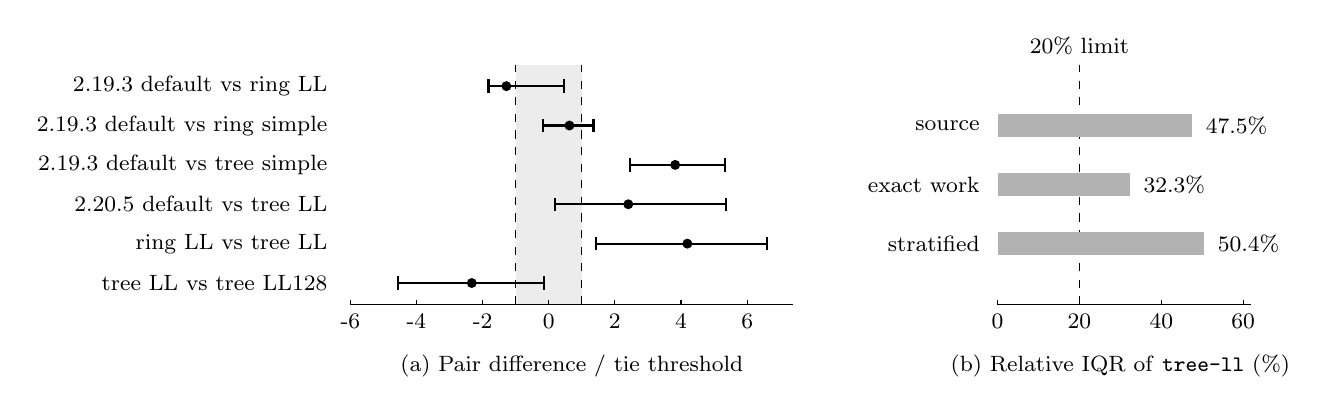
\begin{tikzpicture}[font=\footnotesize]
\begin{scope}[x=0.42cm,y=0.5cm]
\fill[gray!15] (-1,-0.55) rectangle (1,5.55);
\draw[dashed] (-1,-0.55) -- (-1,5.55);
\draw[dashed] (1,-0.55) -- (1,5.55);
\node[below] at (-6,-0.55) {-6};
\draw (-6,-0.55) -- (-6,-0.43);
\node[below] at (-4,-0.55) {-4};
\draw (-4,-0.55) -- (-4,-0.43);
\node[below] at (-2,-0.55) {-2};
\draw (-2,-0.55) -- (-2,-0.43);
\node[below] at (0,-0.55) {0};
\draw (0,-0.55) -- (0,-0.43);
\node[below] at (2,-0.55) {2};
\draw (2,-0.55) -- (2,-0.43);
\node[below] at (4,-0.55) {4};
\draw (4,-0.55) -- (4,-0.43);
\node[below] at (6,-0.55) {6};
\draw (6,-0.55) -- (6,-0.43);
\draw (-6,-0.55) -- (7.4,-0.55);
\node[anchor=east] at (-6.4,5) {2.19.3 default vs ring LL};
\draw[line width=0.8pt] (-1.8238,5) -- (0.4674,5);
\draw[line width=0.8pt] (-1.8238,4.83) -- (-1.8238,5.17);
\draw[line width=0.8pt] (0.4674,4.83) -- (0.4674,5.17);
\fill (-1.2797,5) circle (1.8pt);
\node[anchor=east] at (-6.4,4) {2.19.3 default vs ring simple};
\draw[line width=0.8pt] (-0.1728,4) -- (1.3540,4);
\draw[line width=0.8pt] (-0.1728,3.83) -- (-0.1728,4.17);
\draw[line width=0.8pt] (1.3540,3.83) -- (1.3540,4.17);
\fill (0.6266,4) circle (1.8pt);
\node[anchor=east] at (-6.4,3) {2.19.3 default vs tree simple};
\draw[line width=0.8pt] (2.4487,3) -- (5.3367,3);
\draw[line width=0.8pt] (2.4487,2.83) -- (2.4487,3.17);
\draw[line width=0.8pt] (5.3367,2.83) -- (5.3367,3.17);
\fill (3.8243,3) circle (1.8pt);
\node[anchor=east] at (-6.4,2) {2.20.5 default vs tree LL};
\draw[line width=0.8pt] (0.1916,2) -- (5.3701,2);
\draw[line width=0.8pt] (0.1916,1.83) -- (0.1916,2.17);
\draw[line width=0.8pt] (5.3701,1.83) -- (5.3701,2.17);
\fill (2.4060,2) circle (1.8pt);
\node[anchor=east] at (-6.4,1) {ring LL vs tree LL};
\draw[line width=0.8pt] (1.4320,1) -- (6.5927,1);
\draw[line width=0.8pt] (1.4320,0.83) -- (1.4320,1.17);
\draw[line width=0.8pt] (6.5927,0.83) -- (6.5927,1.17);
\fill (4.1916,1) circle (1.8pt);
\node[anchor=east] at (-6.4,0) {tree LL vs tree LL128};
\draw[line width=0.8pt] (-4.5649,0) -- (-0.1344,0);
\draw[line width=0.8pt] (-4.5649,-0.17) -- (-4.5649,0.17);
\draw[line width=0.8pt] (-0.1344,-0.17) -- (-0.1344,0.17);
\fill (-2.3267,0) circle (1.8pt);
\node at (0.7,-2.1) {(a) Pair difference / tie threshold};
\end{scope}
\begin{scope}[xshift=5.7cm,x=0.052cm,y=0.5cm]
\draw (0,-0.55) -- (62,-0.55);
\node[below] at (0,-0.55) {0};
\draw (0,-0.55) -- (0,-0.43);
\node[below] at (20,-0.55) {20};
\draw (20,-0.55) -- (20,-0.43);
\node[below] at (40,-0.55) {40};
\draw (40,-0.55) -- (40,-0.43);
\node[below] at (60,-0.55) {60};
\draw (60,-0.55) -- (60,-0.43);
\draw[dashed] (20,-0.55) -- (20,5.55);
\node[anchor=south] at (20,5.55) {20\% limit};
\node[anchor=east] at (-2,4.0) {source};
\fill[gray!60] (0,3.70) rectangle (47.4731,4.30);
\node[anchor=west] at (48.4731,4.0) {47.5\%};
\node[anchor=east] at (-2,2.5) {exact work};
\fill[gray!60] (0,2.20) rectangle (32.2775,2.80);
\node[anchor=west] at (33.2775,2.5) {32.3\%};
\node[anchor=east] at (-2,1.0) {stratified};
\fill[gray!60] (0,0.70) rectangle (50.4286,1.30);
\node[anchor=west] at (51.4286,1.0) {50.4\%};
\node at (30,-2.1) {(b) Relative IQR of \texttt{tree-ll} (\%)};
\end{scope}
\end{tikzpicture}
